%%
% This is an Overleaf template for Master's and Bachelor's theses
% using the TUM Corporate Desing https://www.tum.de/cd
%
% For further details on how to use the template, take a look at our
% GitLab repository and browse through our test documents
% https://gitlab.lrz.de/latex4ei/tum-templates.
%
% The tumbook class is based on the KOMA-Script class scrbook.
% If you need further customization please consult the KOMA-Script guide
% https://ctan.org/pkg/koma-script.
% Additional class options are passed down to the base class.
%
% If you encounter any bugs or undesired behaviour, please raise an issue
% in our GitLab repository
% https://gitlab.lrz.de/latex4ei/tum-templates/issues
% and provide a description and minimal working example of your problem.
%%


\documentclass[
  a4paper,            % paper size (a4paper, a5paper)
  english,            % define the document language (english, german)
  % BCOR=5mm,           % define a binding offset for the document
  % coverBCOR=1cm,      % define a different binding offset for the cover page
  % coverpage=false,    % disable the cover page (e.g. if a tumcover is used)
  % titlepage=false,    % disable the additional title page
  % oneside,            % use onesided or twosided layout (oneside, twoside)
  % headmarks=true,     % enable headmarks (true, false)
  % font=times          % define main text font (helvet, times, palatino, libertine)
]{tumbook}

% For theses that are printed with a transparent cover it is recommended to
% use the coverpage and provide the proper coverBCOR, so the distance between
% the binding strip and the content is properly set to 1 * logoheight.
% In this case, the publisher and titleback information is most certainly
% empty and the titlepage may be turned off.
%
% For theses that are printed with a soft cover or by a publisher it is
% recommended to create a cover using the tumcover class and therefore turn
% off the coverpage here. In this case, you most certainly have publisher and
% titleback information and you should keep the titlepage option enabled.


% load additional packages
\usepackage{lipsum}
\usepackage{float}

\usepackage[
    backend=biber,
    style=numeric,
]{biblatex}

\addbibresource{thesis.bib}

% thesis metadata
\title{Circular RNAs in estrogen signaling and breast cancer biology}
\subtitle{Zirkuläre RNAs in der Östrogensignalgebung und der Biologie des Brustkrebses}
\author{Nico Trummer}

\degree{Bachelor of Science (B.Sc.)}
\dateSubmitted{01.04.2021}

\examiner{Prof.\@~Dr.\@ Markus List}
\supervisor{Markus Hoffmann, PhD}


\begin{document}
\setcounter{tocdepth}{4}

\frontmatter
\maketitle
\chapter{Abstract}
\section{Abstract}
The abstract of your thesis goes here.

\lipsum[1-6]

\section{Kurzzusammenfassung}

Deutsche Version des Abstracts.

\lipsum[1-6]
\tableofcontents

\mainmatter
\chapter{Introduction}
\section{Outline}

\begin{itemize}
    \item Describe role of breast cancer in modern health care
    \begin{itemize}
        \item Abundance
        \item Outcomes
    \end{itemize}
    \item Describe current methods for diagnosis and treatment
    \begin{itemize}
        \item Gene panels for risk-assessment of already detected tumors
        \item Shortage of methods for detecting tumors on a molecular basis (need to do more research here)
    \end{itemize}
    \item Describe how circRNAs can improve diagnosis and treatment quality
    \begin{itemize}
        \item Short description of circRNA structure
        \item Increased stability compared to linear RNA biomarkers
        \item Regulatory roles, potential drug targets
        \item Help understanding how well existing treatment methods work (Letrozole, Tamoxifen)
    \end{itemize}
    \item Describe how this thesis approaches the investigation of circRNAs
    \begin{itemize}
        \item Not sure how much detail is necessary here, and how much should be left for materials and methods
    \end{itemize}
\end{itemize}

\section{Introduction}

\lipsum[1-10]

\chapter{Background}
A very high-level overview of the topic is given here.

\lipsum[1]

\section{circRNAs}
This section describes what circRNAs are, how they are formed, and what their functions are.
It also gives insights into the current state of research.

\subsection{Biogenesis}
This subsection describes how circRNAs are formed.

\begin{figure}[H]
    \centering
    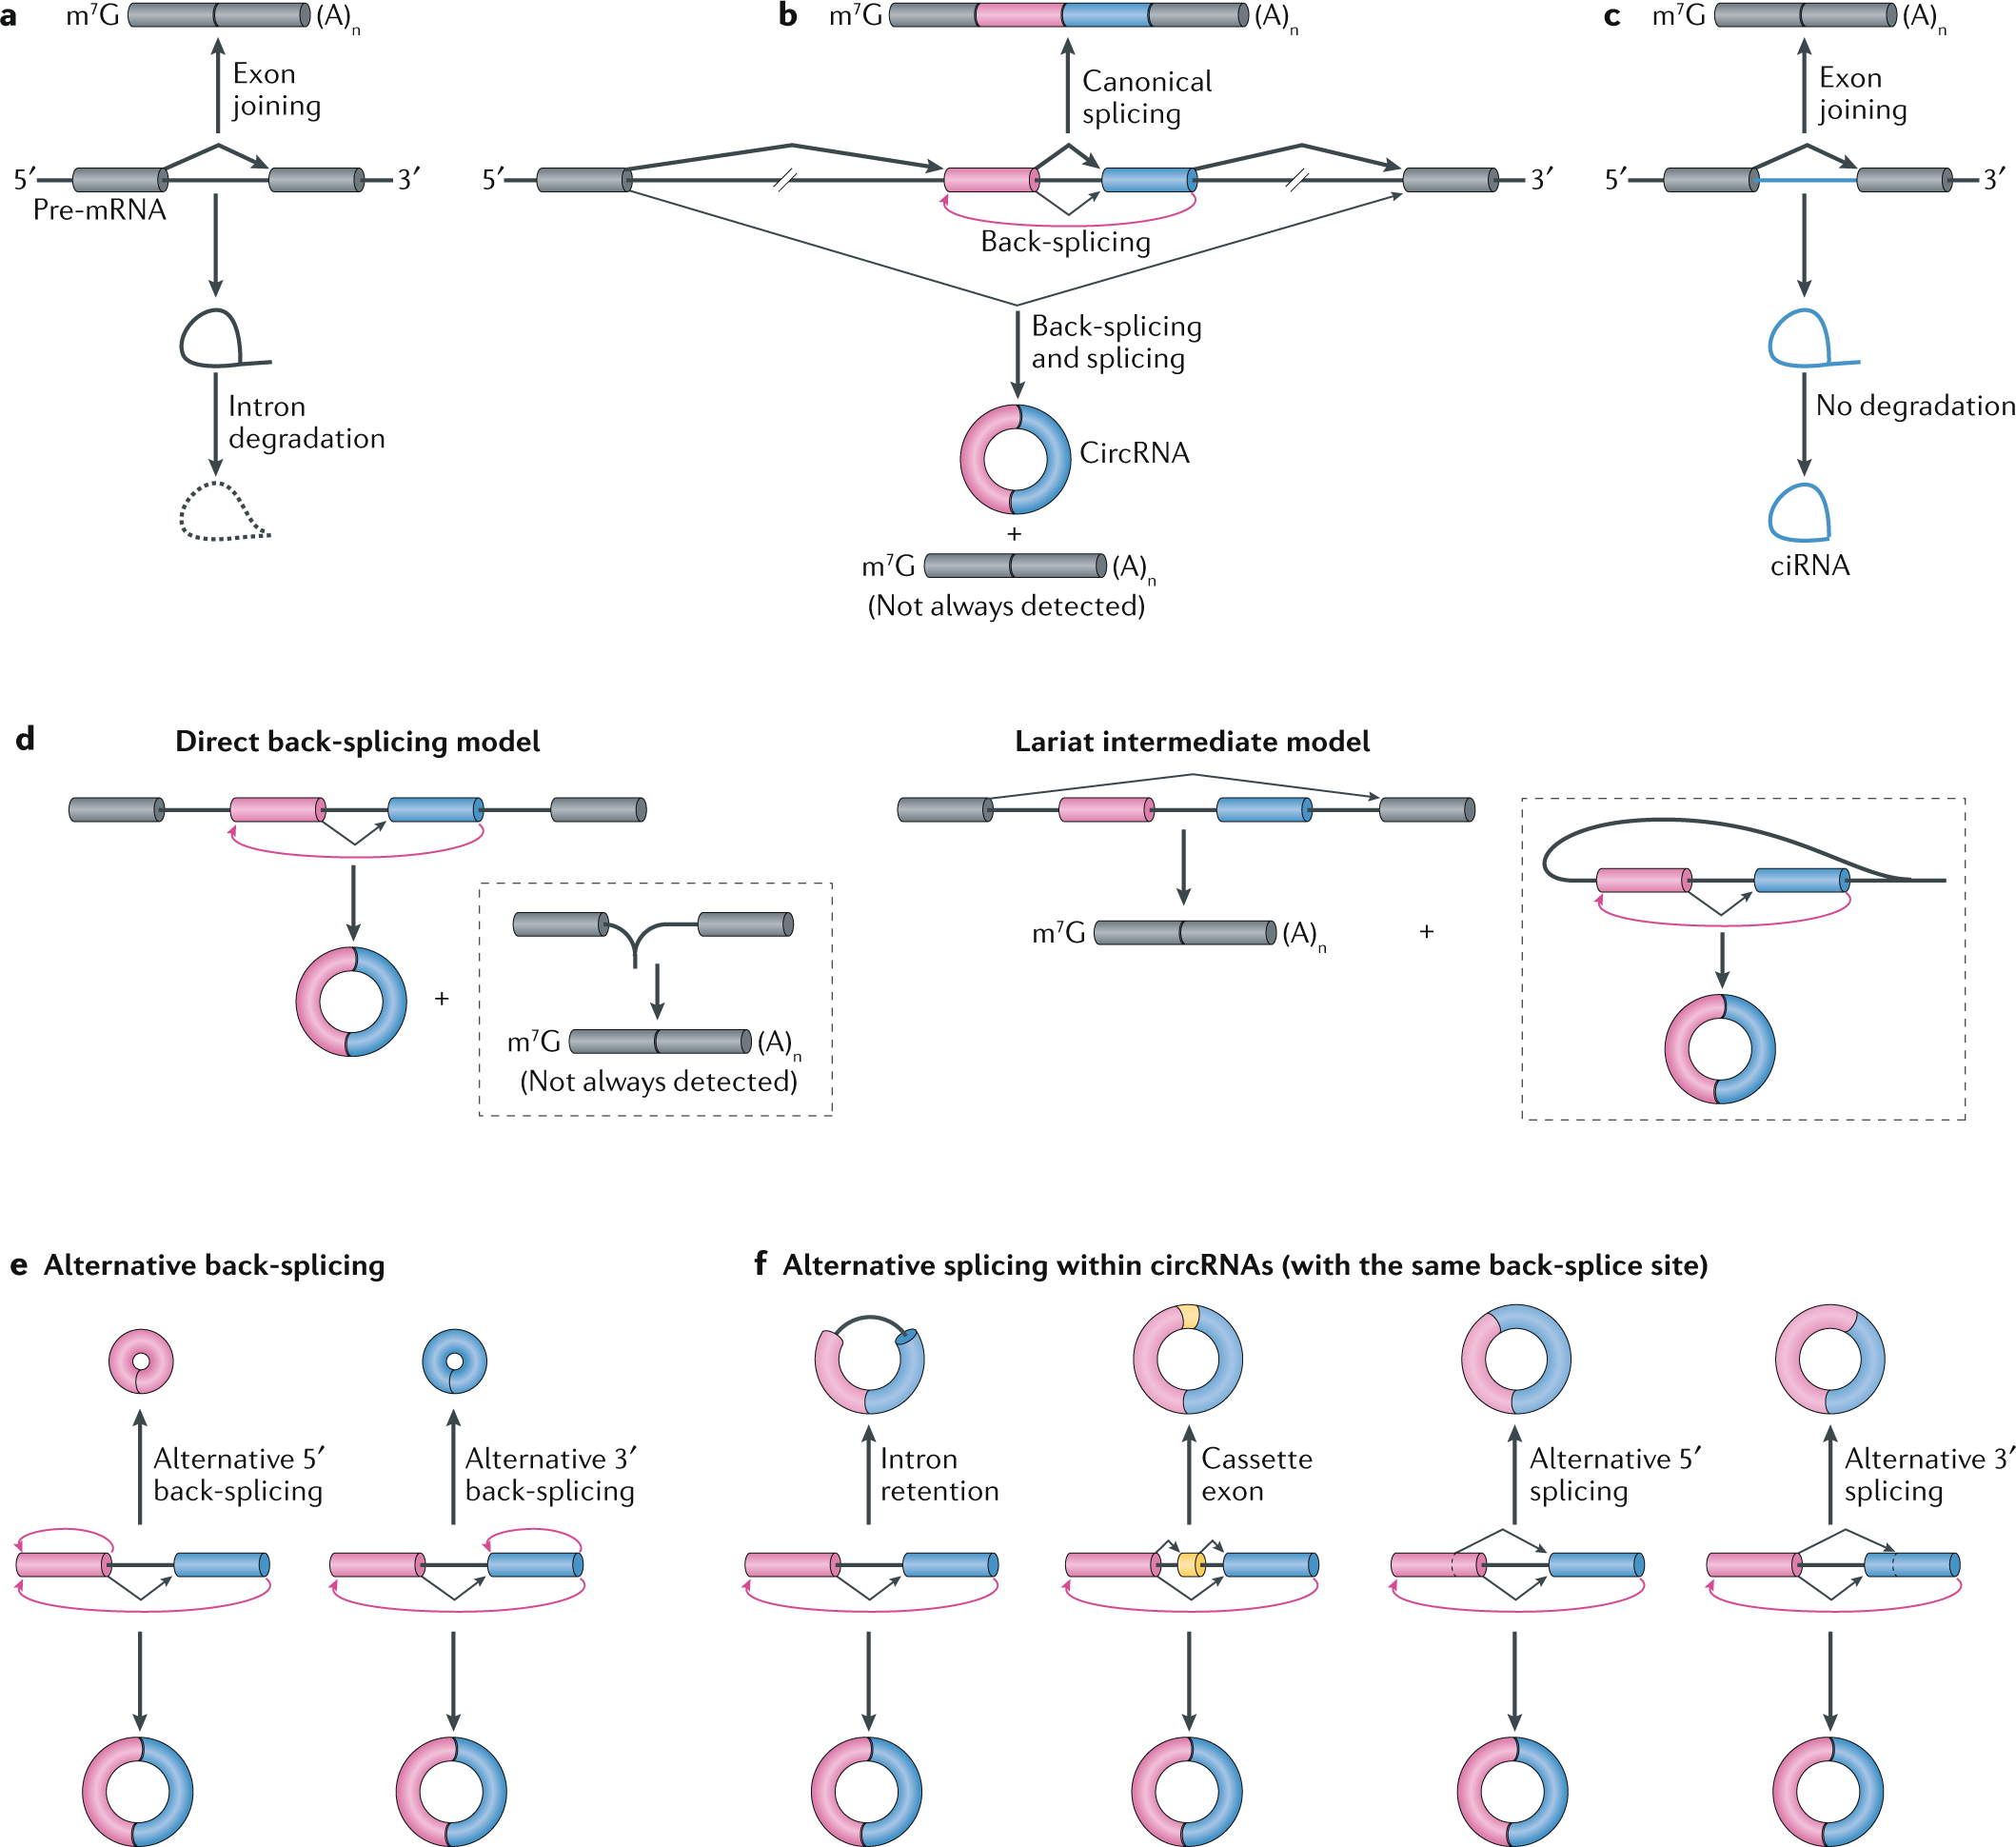
\includegraphics[width=\textwidth]{chapters/background/figures/circRNA-splicing.png}
    \caption{Splicing of circRNAs}
    \label{fig:circRNA_splicing}
\end{figure}

\subsection{Functions}
This subsection describes what functions circRNAs have.

\subsubsection{miRNA sponges}
This subsubsection describes how circRNAs can act as miRNA sponges.

\subsubsection{Protein binding}
This subsubsection describes how circRNAs can bind to proteins.

\subsubsection{Protein coding}
This subsubsection describes how circRNAs can code for proteins.

\subsection{Existing research}
This subsection describes the current state of research on circRNAs.

\section{totalRNA sequencing}
This subsection describes the sequencing method used to identify circRNAs.

\lipsum[2]

\section{Breast cancer}
This section describes what breast cancer is, how it is diagnosed, and what the current treatment options are.
It also gives insights into the current state of research.

\lipsum[3]

\section{Estrogen signaling}
This section describes what estrogen is, how it affects breast cancer, and what the current treatment options are.
It also gives insights into the current state of research.

\lipsum[4]

\section{Related work}
This section describes related work on circRNAs, breast cancer, and estrogen signaling.

\subsection{circRNA-sponging pipeline}
This subsection describes a pipeline for identifying circRNA sponges.

\chapter{Materials and Methods}
\section{nf-core/circrna}
Hello world

\lipsum[1-2]



\chapter{Results and Discussion}
\section{circRNAs associated with estrogen signaling}
Results and discussion

\lipsum[1-2]

\section{The role of inferential uncertainty}
Results and discussion

\lipsum[1-2]


\appendix
\chapter{Appendix}
\lipsum[4]

% \backmatter
% \bibliography{}

\printbibliography

\end{document}
